\documentclass[margin=0mm]{standalone}
\usepackage{tikz}
\usepackage{pgfplots}
 \pgfplotsset{compat=newest}
\usetikzlibrary{math,matrix,fit,positioning}

\usepackage{tikzorbital}

\begin{document}

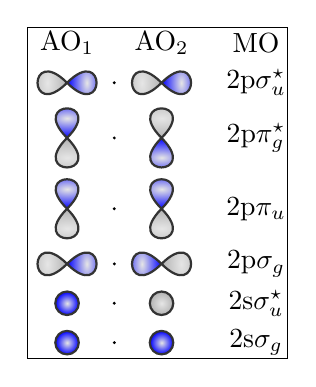
\begin{tikzpicture} 
\useasboundingbox (0.7,-0.2) rectangle (4,4);
\draw (0.7,-0.2) rectangle (4,4);

\tikzmath{ \x1 = 3.6; \x2 = 1.2; \x3 = 2.4; \ps=0.5;}
\tikzmath{ \dy1 = 0.5; \dy2 = 0.9;}

\tikzmath{ \xc = (\x2 + \x3)/2;}
\tikzmath{ \y = 0;}
\node at (\x1,\y) {2s$\sigma_g$};
\orbital[pos = {(\x2,\y)},scale=\ps]{s}
\orbital[pos = {(\x3,\y)},scale=\ps]{s}
\draw  (\xc,\y) circle (0.3pt);

\tikzmath{ \y = \y + \dy1;}
\node at (\x1,\y) {2s$\sigma_u^\star$};
\orbital[pos = {(\x2,\y)},scale=\ps]{s}
\orbital[pos = {(\x3,\y)}, color=black!30,scale=\ps]{s}
\draw  (\xc,\y) circle (0.3pt);

\tikzmath{ \y = \y + \dy1;}
\node at (\x1,\y) {2p$\sigma_g$};
\orbital[pos = {(\x2,\y)},scale=\ps]{py}
\orbital[pos = {(\x3,\y)},scale=\ps]{-py}
\draw  (\xc,\y) circle (0.3pt);


\tikzmath{ \y = \y + (\dy2 + \dy1)/2;}
\node at (\x1,\y) {2p$\pi_u$};
\orbital[pos = {(\x2,\y)},scale=\ps]{pz}
\orbital[pos = {(\x3,\y)},scale=\ps]{pz}
\draw  (\xc,\y) circle (0.3pt);


\tikzmath{ \y = \y + \dy2;}
\node at (\x1,\y) {2p$\pi_g^\star$};
\orbital[pos = {(\x2,\y)},scale=\ps]{pz}
\orbital[pos = {(\x3,\y)},scale=\ps]{-pz}
\draw  (\xc,\y) circle (0.3pt);


\tikzmath{ \y = \y +  (\dy2 + \dy1)/2;}
\node at (\x1,\y) {2p$\sigma_u^\star$};
\orbital[pos = {(\x2,\y)},scale=\ps]{py}
\orbital[pos = {(\x3,\y)},scale=\ps]{py}
\draw  (\xc,\y) circle (0.3pt);

\tikzmath{ \y = \y + \dy1;}
\node at (\x1,\y) {MO};
\node at (\x2,\y) {AO$_1$};
\node at (\x3,\y) {AO$_2$};

%
%
%
%
%\orbital[pos = {(3.5,0)}]{pz}
%
%\orbital[pos = {(3,0)}, scale=2, opacity=0.7]{s}
%
%
%\orbital[pos = {(1,0)}]{-py}
%
%\orbital[pos = {(0.5,0)}, scale=2, opacity=0.7]{s}
%
%\node[below] at (0.8,-0.8) {$A \neq 0$};
%\node[below] at (3.2,-0.8) {$A = 0$};


\end{tikzpicture}



\end{document}